\section{Greedy Problems}

Greedy problems are problems where the optimal solution can always be developed by, at each opportunity, making the choices that provide the most immediate benefit. In other words, the locally optimal choice is also (part of) the globally optimal choice, in all circumstances. Practically, this just means that at any given step of an algorithm, we can reasonably and reliably make the best choice we can.

For example, a simple greedy problem might look like: we are given a binary search tree (remember that elements larger than a given node are always to the right, as a property of binary search trees), and we must print what the maximum element of this tree is.

The greedy solution to this problem is to always traverse to the right of the tree until we end up at a leaf node. This leaf node is the largest element of the tree, guaranteed by the properties of a binary search tree. In greedy terms, starting from the root of the tree, we will greedy move to the largest child node.

{\centering 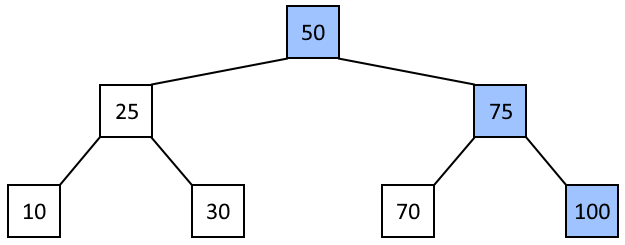
\includegraphics{images/greedy/greedy_tree_1.png}}

In the above example, we can easily verify that 100 is the largest element in the binary search tree.

We can show a similar but slightly modified problem that stops being greedy: we are given a binary tree (that isn't necessarily a binary search tree), and we must print what the maximum element of this tree is.

Here, this is problem is no longer greedy because we can't reliably say that the largest element is always a child of the larger node at each step. Our greedy solution only worked because we could be guaranteed, at each decision, that our locally optimal choice would lead us to the global optimal.

{\centering 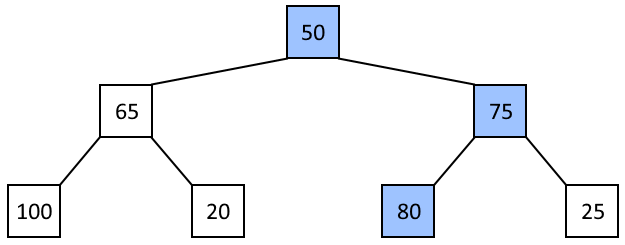
\includegraphics{images/greedy/greedy_tree_2.png}}

While in this case we do greedily take the locally optimal choice at each step, the globally optimal answer involves us taking the locally sub-optimal choice of 65 instead of 75. Because we're not dealing with a binary search tree, we don't have the guarantees we need to greedily approach this problem.

\subsection{Knapsack}

\subsection{Coin Change}

\subsection{Interval Cover}